\setlength{\abovedisplayskip}{-25pt}
\setlength{\belowdisplayskip}{-25pt}

\section{Análise Teórica}

\subsection{Retificador de meia onda de precisão}

Para a análise do retificador de precisão de meia onda (circuito da figura \ref{ckt:1}), conhecendo anteriormente como um amplificador operacional e diodos funcionam, devemos separar duas relações entre a entrada e a saída de interesse:

\begin{itemize}
    \item Para o caso $V_{in}>0$ \\
    \begin{center}
        \begin{equation} \label{vsat+}
            V_{out} = 0
        \end{equation}
    \end{center}
    
    \item Para o caso $V_{in}<0$ \\ 
    
    \begin{center}
        \begin{equation} \label{vsat+}
            V_{out} = -\frac{R_f}{R_1}\times V_{in}
        \end{equation}
    \end{center}
\end{itemize}

É importante notar que o circuito para o caso $V_{in}<0$ funciona como um amplificador inversor, pois o diodo que se encontra entre a saída e a entrada inversora está em corte e o diodo da saída está em condução com uma malha negativa no AMPOP.

Como as resistências de entrada e saída são exatamente as mesmas ($1.2\times10^3$  \ohm), logo teremos para o caso em que $V_{in}<0$, uma saída de $V_{out}=-V_{in}$.

Desenhando a característica de transferência do circuito da figura \ref{ckt:1}, teremos.

\begin{figure}[H]
\begin{center}
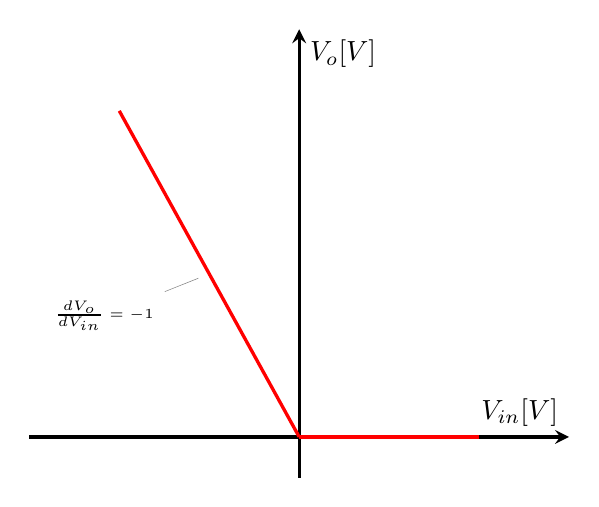
\begin{tikzpicture} 
\begin{axis}[very thick,
                     samples = 100,
                     ytick={-10,10},
                     xlabel = {$V_{in}[V]$},
                     ylabel = {$V_{o}[V]$},
                     xmin = -6,
                     xmax = 6,
                     ymin = -0.5,
                     ymax = 5,
                     axis x line = middle,
                     axis y line = middle,
                     ticks = none]
            \addplot[draw=red, domain=-4:0] plot (\x, {-\x});
            \addplot[draw=red, domain=0:4] plot (\x, {0});
            \addplot[mark=none] coordinates {(-2,2)} node[pin=200:{\tiny $\frac{dV_o}{dV_{in}}=-1$}]{};
        \end{axis}
\end{tikzpicture}
\end{center}
\caption{Característica de transferência para o retificador de meia onda de precisão.}
\label{graph:1} 
\end{figure}

Pela CT acima, espera-se que a parte negativa do sinal seja retificada e invertida.

Como foi colocado uma onda com $0.5V_{pico}$, espera que os resultados práticos sejam os mesmos com amplitude máxima do sinal de saída de aproximadamente $0.5V_{pico}$ quando a entrada se encontra em $-0.5V_{pico}$ após a retificação. Como pode ser visto abaixo na simulação do LTSpice.

\begin{figure}[H] 
\centering
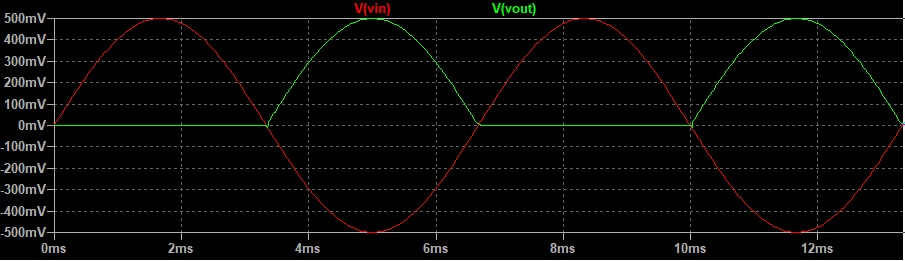
\includegraphics[scale=0.6]{images/vo_1.jpg}
\caption{Simulação da entrada e saída do retificador de meia onda.}
\label{fig1} 
\end{figure}

\subsection{Retificador de onda completa de precisão}

Semelhantemente para o circuito da figura \ref{ckt:2}, teremos que analisar a relação da entrada com a saída para dois casos diferentes.

\begin{itemize}
    \item Para o caso $V_{in}>0$ \\
    \begin{center}
        \begin{equation} \label{vsat+}
            V_{out} = \frac{R_2 \times R_5 }{R_1 \times R_4} \times V_{in} = \alpha \times V_{in}
        \end{equation}
    \end{center}
    
    \item Para o caso $V_{in}<0$ \\
    
    \begin{center}
        \begin{equation} \label{vsat+}
            V_{out} = -\frac{R_3}{R_1} \times \frac{R_2 + R_4 + R_5}{R_2 + R_3 + R_4} \times V_{in} = -\beta \times V_{in}
        \end{equation}
    \end{center}
\end{itemize}

Temos para o primeiro caso em que $V_{in}>0$, um circuito equivalente de dois inversores, pois não temos o ramo da resistor $R_3$, já que o mesmo não possui corrente, além que o diodo que vai para esse ramo está em corte. Com isso obtemos a expressão mostrada. Já para o segundo caso ($V_{in}<0$), teremos teremos um circuito equivalente a um inversor em cascata com um não-inversor, já que o primeiro diodo se encontra em corte, obtendo a expressão mostrada anteriormente.

Chamando $\alpha$ o ganho relativo ao primeiro caso, e $\beta$ o ganho relativo ao segundo caso.

Onde:
    \begin{center}
        \begin{equation} \label{vsat+}
            \alpha = \frac{R_f}{R_1}
        \end{equation}
    \end{center}
    
\vspace{10pt}
  \begin{center}
        \begin{equation} \label{vsat+}
            \beta = \frac{R_3}{R_1} \times \frac{R_2 + R_4 + R_5}{R_2 + R_3 + R_4}
        \end{equation}
  \end{center}

Como $R_2 = R_3 = R_4 = R_5 = R$, portanto teremos \\

\begin{center}
        \begin{equation} \label{vsat+}
            \alpha = \beta = \frac{R}{R_1} = \frac{12\times 10^3}{6.8\times 10^3} = 1.7647
        \end{equation} 
  \end{center}
 A CT do cicuito da figura \ref{ckt:2} é mostrado abaixo
 
 \begin{figure}[H]
\begin{center}
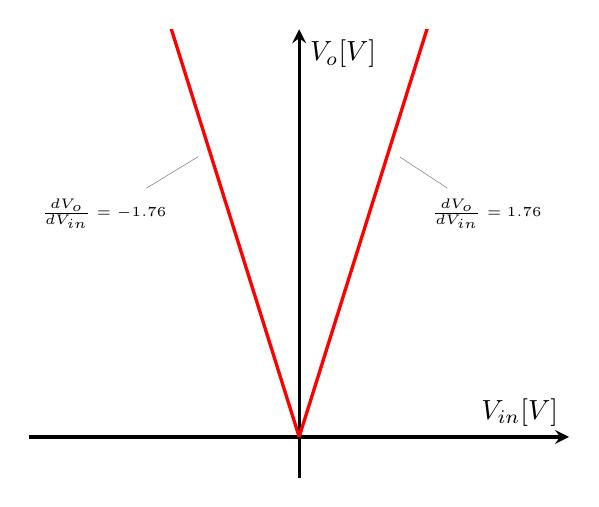
\begin{tikzpicture} 
\begin{axis}[very thick,
                     samples = 100,
                     ytick={-10,10},
                     xlabel = {$V_{in}[V]$},
                     ylabel = {$V_{o}[V]$},
                     xmin = -6,
                     xmax = 6,
                     ymin = -0.5,
                     ymax = 5,
                     axis x line = middle,
                     axis y line = middle,
                     ticks = none]
            \addplot[draw=red, domain=-4:0] plot (\x, {-1.76*\x});
            \addplot[draw=red, domain=0:4] plot (\x, {1.76*\x});
            \addplot[mark=none] coordinates {(-2,3.52)} node[pin=230:{\tiny $\frac{dV_o}{dV_{in}}=-1.76$}]{};
            \addplot[mark=none] coordinates {(2,3.52)} node[pin=-50:{\tiny $\frac{dV_o}{dV_{in}}=1.76$}]{};
        \end{axis}
\end{tikzpicture}
\end{center}
\caption{Característica de transferência para o retificador de onda completa de precisão.}
\label{graph:2} 
\end{figure}
 
 Para uma entrada de $0.5V_{pico}$, teremos uma saída ($V_{out}$) de aproximadamente $0.8824V_{pico}$, onde o circuito é retificado e invertido para valores de entrada negativo, e apenas amplificado para valores de entrada positivo.
 
Em relação a $V_{o1}$, pela a análise do circuito temos:

\begin{itemize}
    \item Para o caso $V_{in}>0$ \\
    \begin{center}
        \begin{equation} \label{vsat+}
            V_{o1} = 0 
        \end{equation}
    \end{center}

    \item Para o caso $V_{in}<0$ \\
    
    \begin{center}
        \begin{equation} \label{vsat+}
            V_{o1} = -\frac{R_3||(R_2+R_4)}{R_1} \times V_{in} = -\frac{R_3 \times (R_2+R_4)}{R_1 \times(R_2 + R_3 + R_4)}\times V_{in}
        \end{equation}
    \end{center}
\end{itemize}

No primeiro caso, como o AMPOP da saída está configurado como amplificador inversor, logo teremos pela realimentação negativa e sabendo que $V^= 0$, devido não percorrer corrente em $R_3$, por essa conclusão obtemos  $V_{o1} = V^+ = V^- = 0$.

Para o segundo caso, como o primeiro AMPOP trabalha como amplificador inversor, a sua saída é $V_{o1}$, pelo o circuito equivalente fornecido.

Para uma entrada de $0.5V_{pico}$ teremos um $V_{o1}$ de: \\

\begin{center}
        \begin{equation} \label{vsat+}
            V_{o1} = -\frac{12\times10^3 (24\times10^3)}{6.8\times10^3(36\times10^3)}\times 0.5 = 0.5882 V_{pico}
        \end{equation}
    \end{center}
    

Fazendo as simulações no LTSpice obtemos os sinais de $V_{out}$ e $V_{o1}$.

\begin{figure}[H] 
\centering
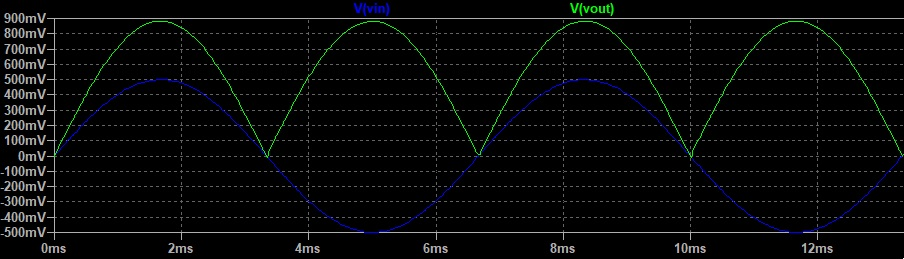
\includegraphics[scale=0.6]{images/vo_2.jpg}
\caption{Simulação da entrada e saída ($V_{out}$) do retificador de onda completa.}
\label{fig1} 
\end{figure}

\begin{figure}[H] 
\centering
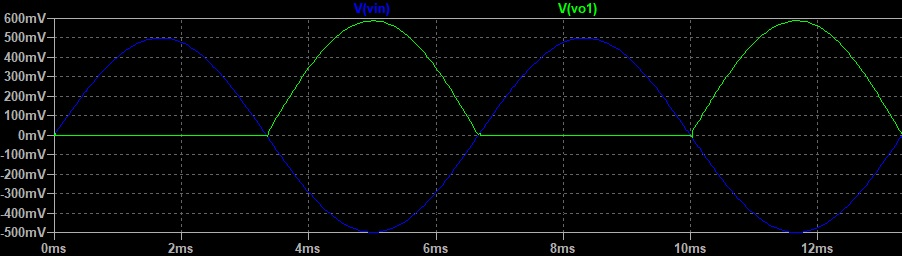
\includegraphics[scale=0.6]{images/vo_3.jpg}
\caption{Simulação da entrada e saída ($V_{o1}$) do retificador de onda completa.}
\label{fig1} 
\end{figure}